\documentclass[../algorithms.tex]{subfiles}
\begin{document}
This chapter is used to conclude all the algorithms and data structures relation by showing examples. For example, we show how we can model this problem using different data structure and end up solving this problem with different algorithms. For some example, we should how different algorithm matters. 
\section{Complete Search VS Smart Search VS Dynamic Programming}
\begin{examples}
\item \textbf{956. Tallest Billboard (hard).} You are installing a billboard and want it to have the largest height.  The billboard will have two steel supports, one on each side.  Each steel support must be an equal height. You have a collection of rods which can be welded together.  For example, if you have rods of lengths 1, 2, and 3, you can weld them together to make a support of length 6. Return the largest possible height of your billboard installation.  If you cannot support the billboard, return 0.
\begin{lstlisting}[numbers=none]
Example 1:

Input: [1,2,3,6]
Output: 6
Explanation: We have two disjoint subsets {1,2,3} and {6}, which have the same sum = 6.

Example 2:

Input: [1,2,3,4,5,6]
Output: 10
Explanation: We have two disjoint subsets {2,3,5} and {4,6}, which have the same sum = 10.

Example 3:

Input: [1,2]
Output: 0
Explanation: The billboard cannot be supported, so we return 0.
\end{lstlisting}
Note: 0 <= rods.length <= 20, 1 <= rods[i] <= 1000. The sum of rods is at most 5000.

\textbf{Solution 1: Naive Complete Search.} We need to have two billboard: left and right side. Given a state (x, y), which means the sum of left and right billboard is x and y respectively. Now, to add a new rod v into the state, we have three options: 1) not use v, (x, y); 2) put v to left side: (x+v, y); 3) put v to the right side (x, y+v). If x' and y' end up to be equal, we can track the maximal value. Given the array size of n, and initial state (0, 0), we use search, each state will have three branches because of the three options, therefore, the state transfer graph(tree) will expand to $\sum(3^0, 3^1, 3^2, ..., 3^{n}) = 3^{n+1}-1$. The code is:
\begin{lstlisting}[language=Python]
def tallestBillboard(self, rods):
    if not rods:
        return 0
    n = len(rods)
    def helper(i, l, r, ans):
        if l == r: 
            ans[0] = max(ans[0], l)
        if i == n:
            return
        helper(i+1, l, r, ans)
        helper(i+1, l+rods[i], r, ans)
        helper(i+1, l, r+rods[i], ans)
        return
    ans = [0]
    helper(0, 0, 0, ans)
    return ans[0]
\end{lstlisting}
\textbf{Solution 2: Smart Complete Search.} Similar to Bidirectional Search, which decrease the time complexty from $n$ power to $n/2$ by starting searching simulatously from soure and goal, and save the final nodes, and its path length from its starting node. The total length can be obtained by the common final nodes (its complexity depends on its total number of states), and sum up its path length of each side. For this problem, we can do the same by dividing the array into half and half. In each half, we enumerate all possible states and save them in a dictionary. If we have (x, y) in the left, and (y, x) in the right, then we have a possible value, which is $x+y$.  In this problem, we can compress the states: assume we have state (x, x+d) and (y, y+d), x < y, the optimal value will always be decided by the second set (y, y+d), therefore, instead of saving all possible (x,y), we can save it as (x-y) and the value is the maximum left length.  
\begin{lstlisting}[language=Python]
def tallestBillboard(self, rods):
    def make(A):
        # enumerate all possible states
        states = {(0, 0)}
        for x in A:
            states |= ({(a+x, b) for a, b in states} |
                       {(a, b+x) for a, b in states})
        # compress states
        delta = {}
        for a, b in states:
            delta[a-b] = max(delta.get(a-b, 0), a)
        return delta
    N = len(rods)
    Ldelta = make(rods[:N//2])
    Rdelta = make(rods[N//2:])

    # meet in the middle
    ans = 0
    for d in Ldelta:
        if -d in Rdelta:
            ans = max(ans, Ldelta[d] + Rdelta[-d])
    return ans
\end{lstlisting}
\textbf{Snapsack\_based Dynamic Programming.}  In this solution, we define a two-dimensional dp array, dp[i][j] means using the first i rods to get a difference j which is the $y-x$. The saved value is the maximum common height for states with the same difference.  The time complexity is bounded by $O(21\times 5000)$. This is similar to the snapsack problem, the difference is within the state transfer function as shown in Fig~\ref{fig:dp_956}. 
\begin{figure}[h]
    \centering
    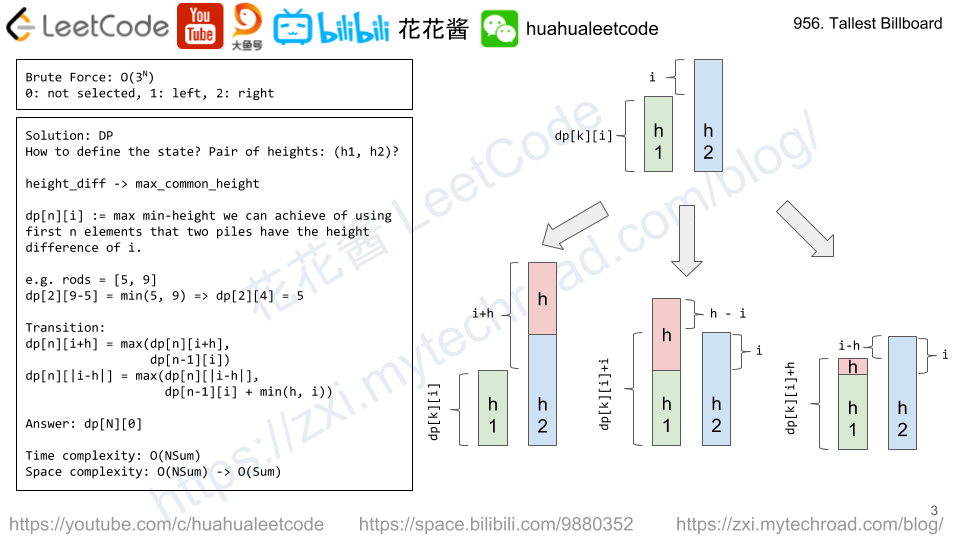
\includegraphics[width=0.9\columnwidth]{fig/956-ep234.png}
    \caption{Dynamic Programming}
    \label{fig:dp_956}
    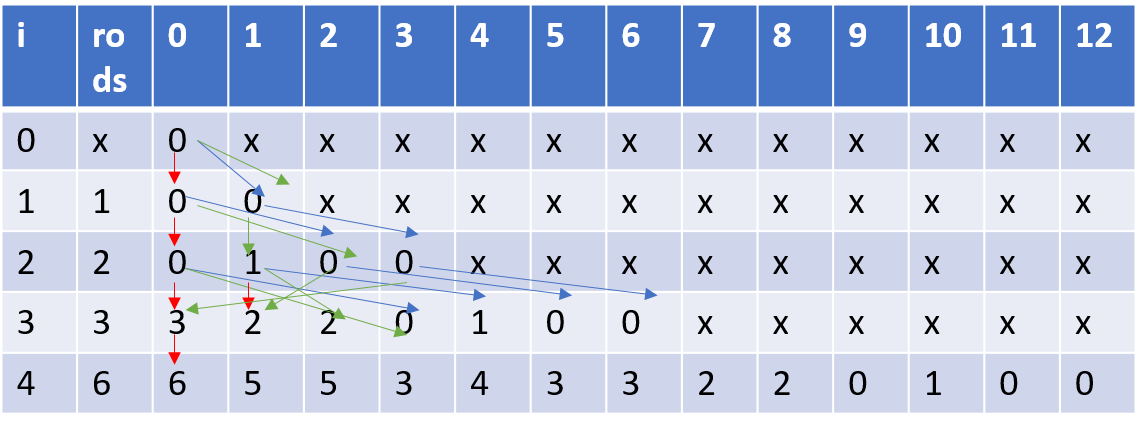
\includegraphics[width=0.9\columnwidth]{fig/956_dp_table.png}
    \caption{The dp table: the arrows of different color means different operation. Red: not use current item, copy from the previous state; Blue: put the item on the taller side, the result is not affected; Green: put the item at the shorter side. }
    \label{fig:dp_956_2}
\end{figure}
\begin{lstlisting}[language=Python]
 def tallestBillboard(self, rods):
    maxHeight = sum(rods)
    maxRods = len(rods)
    dp = [float('-inf') for c  in range(maxHeight+1)]  # use difference
    dp[0] = 0
    for i in range(0, maxRods):
        old_dp = dp[:] 
        for j in range(0, maxHeight+1-rods[i]):
            if old_dp[j] < 0:
                continue
            # green arrow
            if j >= rods[i]:
                dp[j-rods[i]] = max(dp[j-rods[i]], old_dp[j]+min(rods[i], j))
            else:
                dp[rods[i]-j] = max(dp[rods[i]-j], old_dp[j]+min(rods[i], j))
            # blue arrow
            dp[j+rods[i]] = max(dp[j+rods[i]], old_dp[j])                
            # the red line is saved in dp indirectly
    return dp[0]
\end{lstlisting}
\end{examples}
\end{document}